% ***********************************************************************************
% Pure LaTeX part to be inserted in a document (be careful of depencies of packages & commands
% Prepared by XXX and YYY under the supervision of Arnaud de La Fortelle
% Fall 2017
% 2D wave propagation subsection of the modeling part
% ***********************************************************************************


\paragraph{Control model}

We consider here the simplest model for which a Kalman filter can really bring an added value: a linear, Gaussian and real (i.e. 1D) model:
\begin{eqnarray}
\label{kalman-dynamics.eq1}
x_{k+1} &=& A x_k + B u_k + v_k\\
\label{kalman-dynamics.eq2}
y_k &=& C x_k + w_k
\end{eqnarray}
where $X=(x_k)$ is the state of the system (typically a distance to a prescribed value, in whatever unit), $U=(u_k)$ is the control, $Y=(y_k)$ is the measurement. $V=(v_k)$ (resp. $W=(w_k)$) is a Gaussian noise: the $v_k$ (resp. $w_k$)are independent and identically distributed random variables with 0 mean and variance $Q$ (resp. $R$). The initial state $x_0$ is also a centered random variable with variance $\bar{P}_O$. Note that these notation perfectly adapt to multidimensional systems, with matrices: see any textbook on control to get the matrix equations.

This is not specifically needed for Kalman filter, but the usual optimization criteria is quadratic:
\begin{equation}\label{kalman-cost.eq1}
	J(X,U) = \frac{1}{N}\sum_{k=0}^N \alpha u_k^2 + \beta x_k^2
\end{equation}

The Equations~(\ref{kalman-dynamics.eq1})-(\ref{kalman-dynamics.eq2}) are often written for each time step so the scaling with respect to time has to be careful. In a system with a 100 Hz time step (also refered to as control frequency), typical values are:
\begin{eqnarray*}
A &=& 1.001\\
B &=& .01\\
C &=& 1\\
Q &=& .001\\
R &=& .01
\end{eqnarray*}
We have taken $C=1$ because most of the time we try to have a measurement as close to the state as possible and if $C\neq 1$ it is possible to compensate it. $A>1$ means that the system is unstable: Figure~\ref{Kalman-free.fig} shows the divergent behavior.

\begin{figure}[htb]
	\centering
	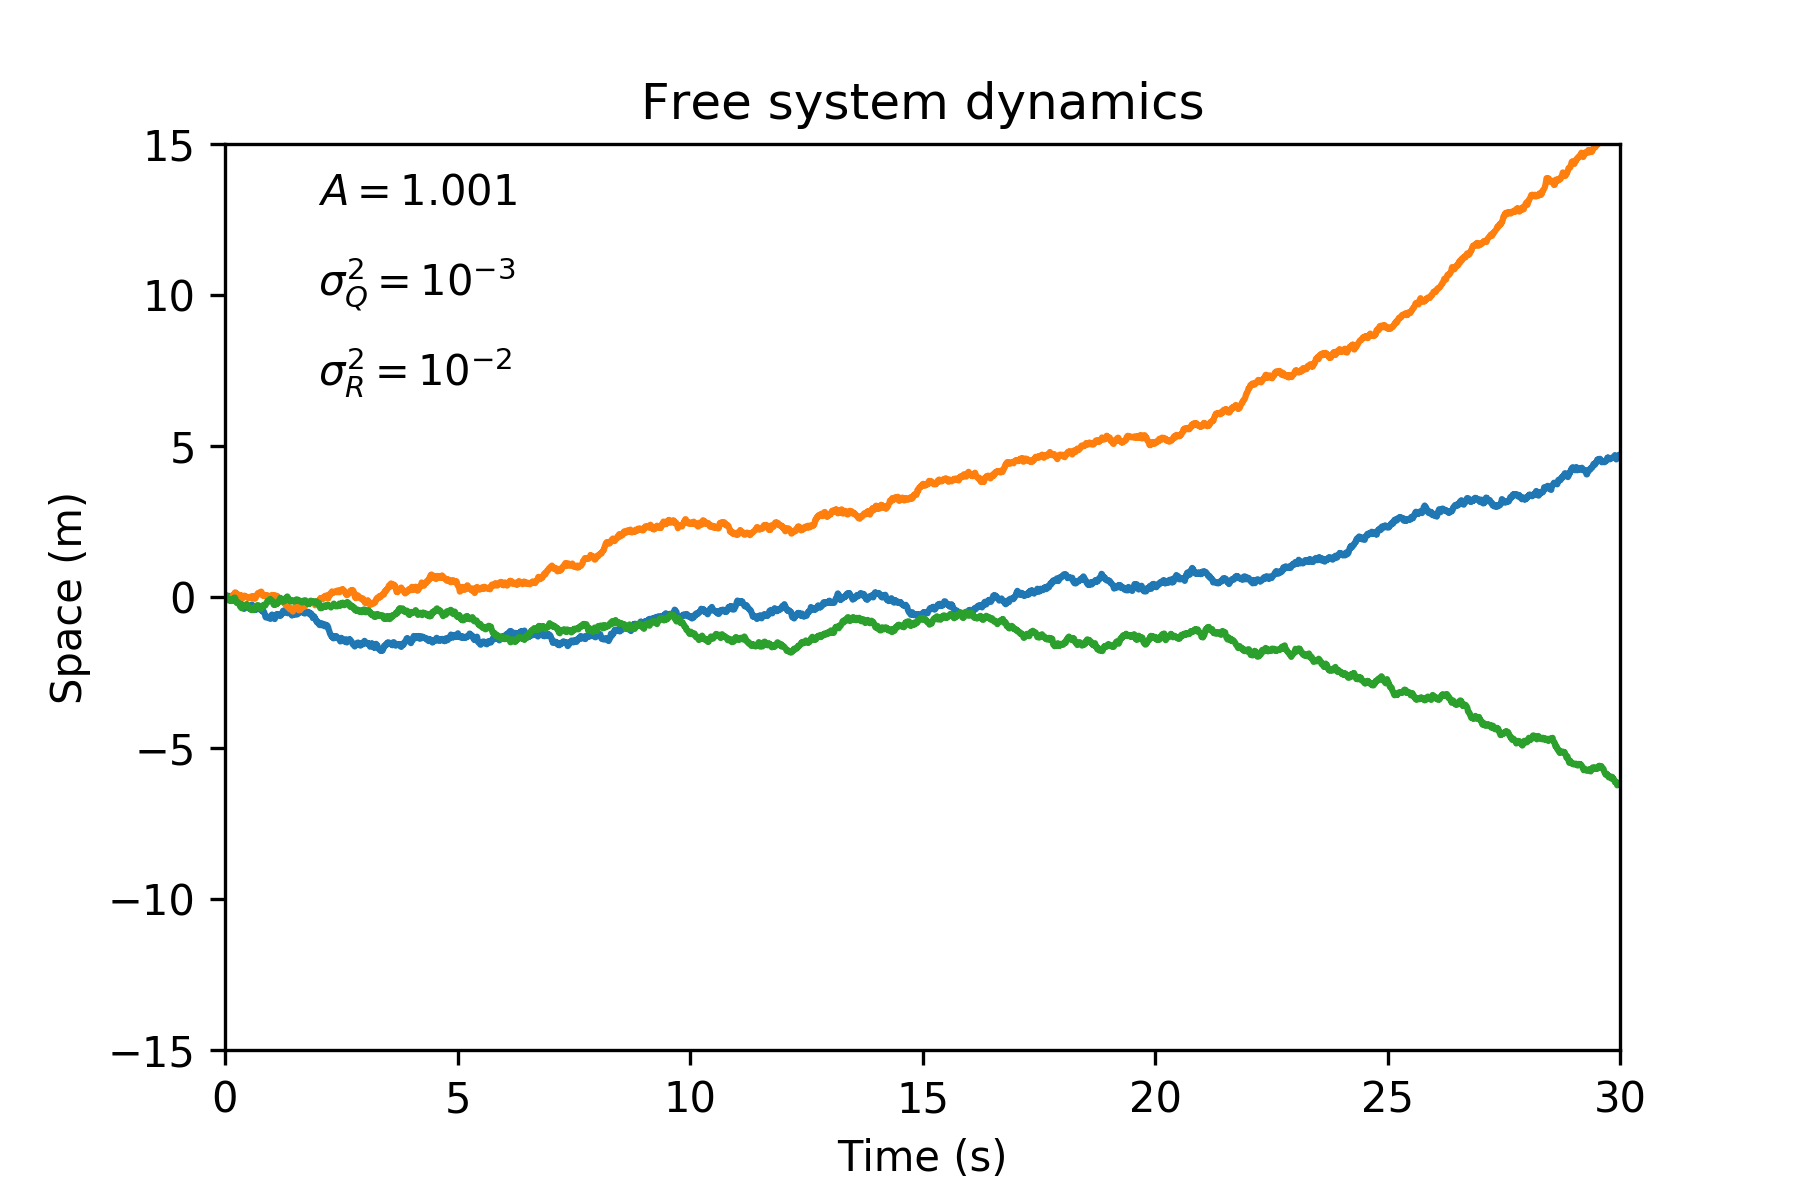
\includegraphics[width=10cm]{Kalman-free}       
	\caption{The free system dynamics: it shows instability and the system tends to diverge exponentially. The variance $\sigma_R^2$ (resp. $\sigma_Q^2$ ) is denoted by $R$ (resp. $Q$) in the system model.}
	\label{Kalman-free.fig}
\end{figure}

\paragraph{A naive control}
Now, we would like to stabilize the state of the system as close to zero as possible, and if possible at a reasonable cost. This means we can adjust the weights $\alpha$ and $\beta$ in the cost function~(\ref{kalman-cost.eq1}). Or simpler measure the 2 partial cost functions
\begin{eqnarray}
\label{kalman-costX.eq}
J_1(X) &=& \frac{1}{N}\sum_{k=0}^N  x_k^2\\
\label{kalman-costU.eq}
J_2(U) &=& \frac{1}{N}\sum_{k=0}^N u_k^2
\end{eqnarray}

Now, we introduce the simplest possible control: a proportional control with gain $K$ defined by:
\begin{equation}
\label{kalman-Pcontrol.eq}
	u_k = -K y_k
\end{equation}

Since we have "unit" parameters, let's start with a unit gain $K=1$. This indeed stabilizes the system as we see in Figure~\ref{Kalman-control-Gain1.fig}.

\begin{figure}[htb]
	\centering
	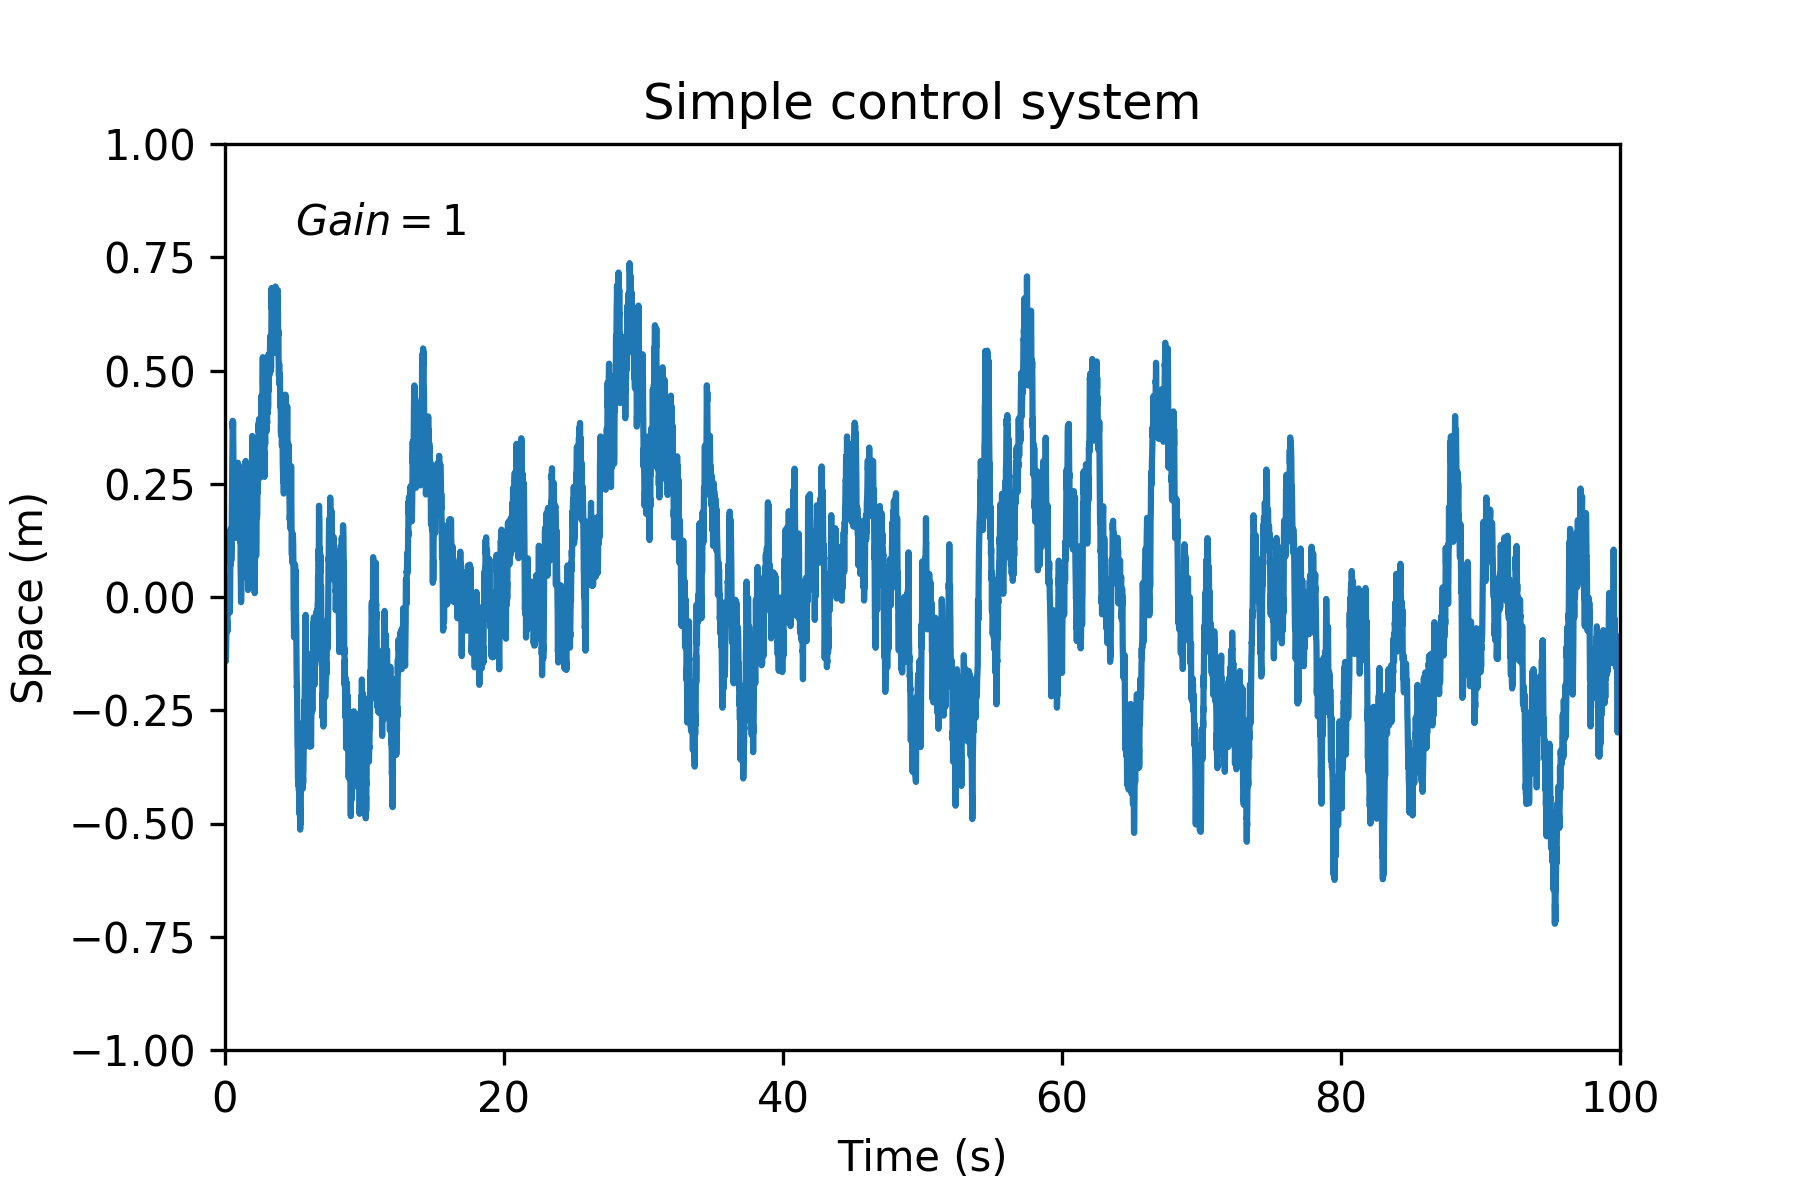
\includegraphics[width=10cm]{Kalman-control-Gain1}       
	\caption{The same system as in Figure~\ref{Kalman-free.fig} with the proportional control as defined by Equation~(\ref{kalman-Pcontrol.eq}) with gain $K=1$. The system is indeed stable with empirical costs $J_1=0.06$ and  $J_2=0.07$.}
	\label{Kalman-control-Gain1.fig}
\end{figure}

Now, if we try to maximize the precision (at all cost), we can try to compensate the term $A x_k$ in Equation~(\ref{kalman-dynamics.eq1}) by the term $B u_k = -BK Y_k = -(BKC) x_k -BK w_k$. Since we have no control onto the noise, and since this noise is centered, let's take $A = BKC$, i.e. in our case $K = A/BC = 100.1$. This lead to the result of Figure~\ref{Kalman-control-Gain100.fig}. What is impressive is not so much the increase in precision, $J_1$ is divided by about 5, that the explosion of the control cost $J_2$, multiplied by about 3,000.

\begin{figure}[htb]
	\centering
	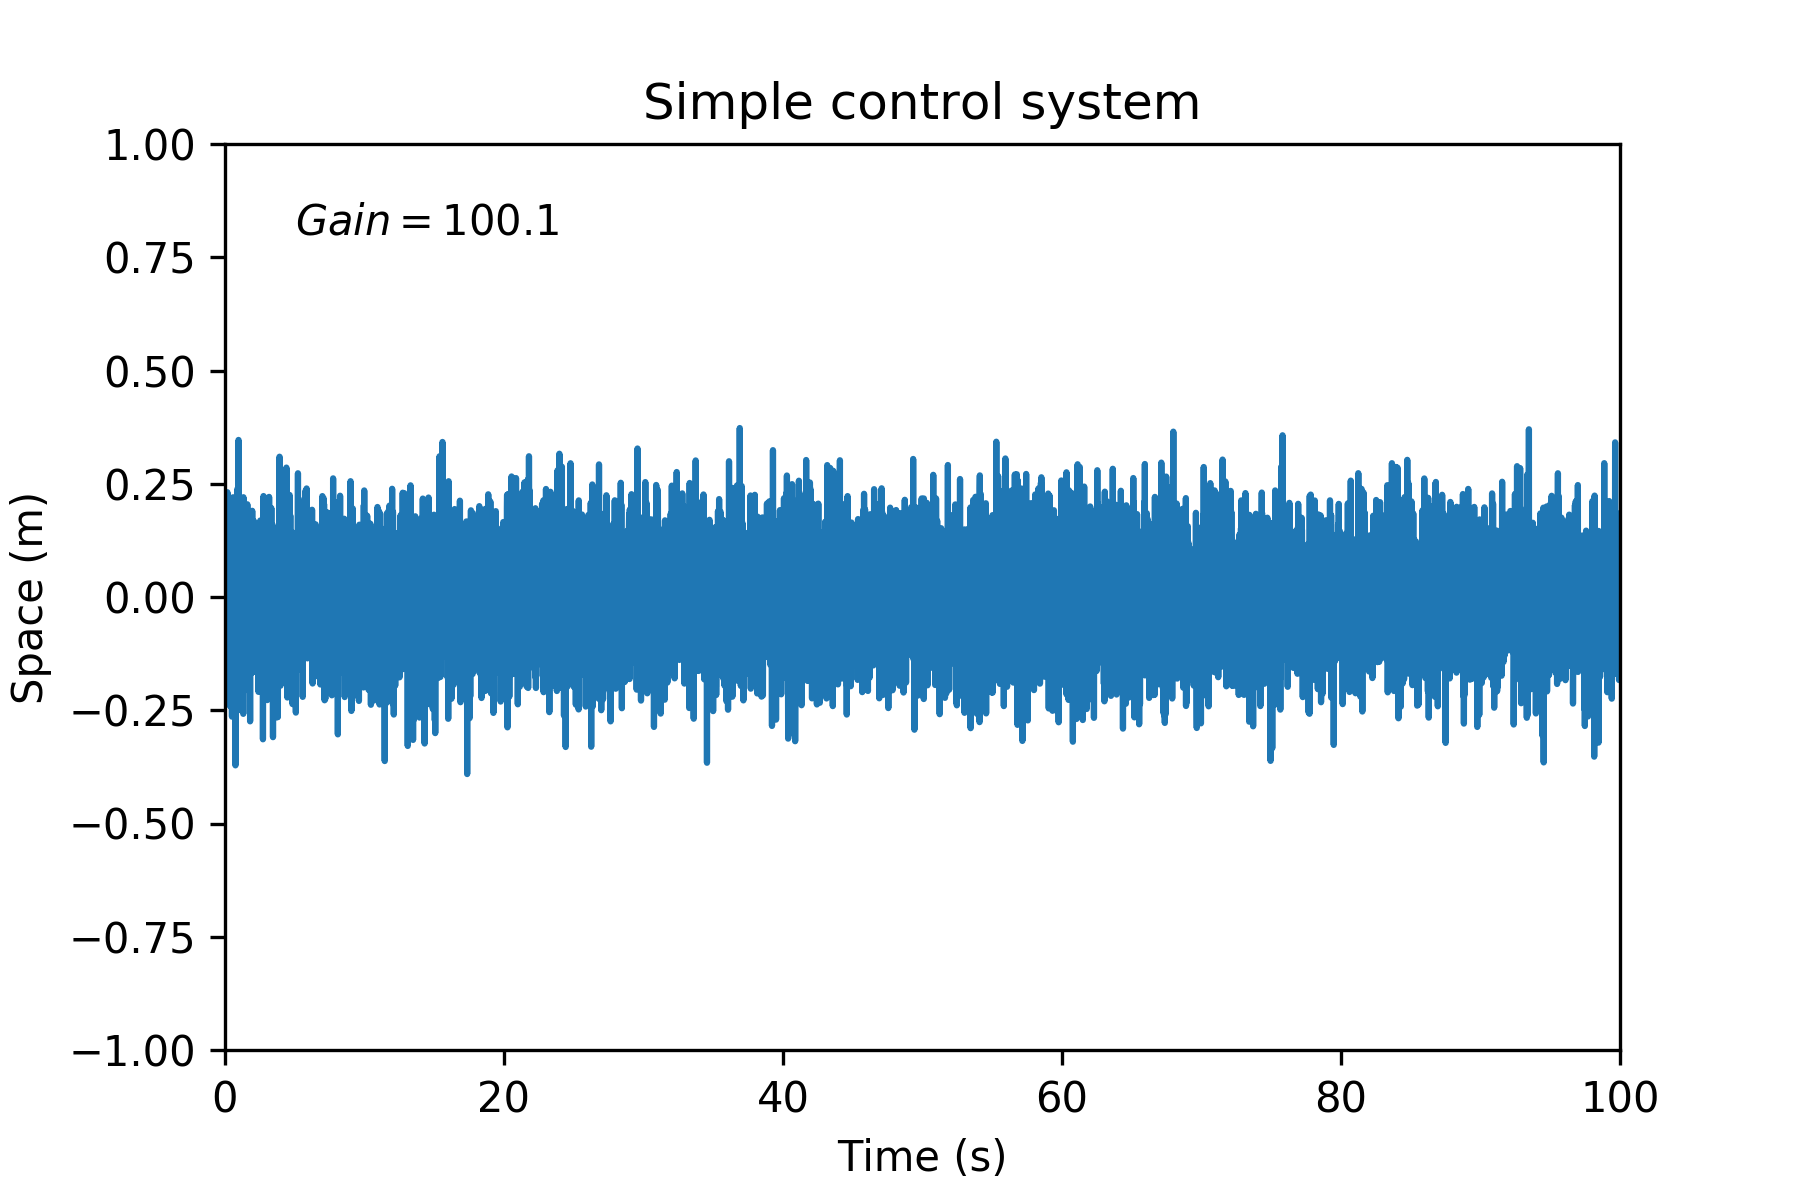
\includegraphics[width=10cm]{Kalman-control-Gain100}       
	\caption{The same system as in Figure~\ref{Kalman-control-Gain1.fig} with $K=100.1$ in order to fully compensate $A$. The system is very stable with empirical costs $J_1=0.011$ and  $J_2=209$.}
	\label{Kalman-control-Gain100.fig}
\end{figure}

In order to learn more about the trade-off between precision and control cost, one can test intermediary gains, and for $K=10$, we get the Figure~\ref{Kalman-control-Gain10.fig}. There we have a surprise: the precision is better than with our naively optimal gain $K=100.1$, not to speak of the decrease of the control cost. There are now 2 paths for us: either --- pragmatically --- adjust the gain to get the best control, or --- analytically --- try to understand what was wrong. Indeed, this numerical experiment clearly shows we are missing an important idea. And the idea we are missing is the following: we can have much better estimates of $x_k$ than $y_k$ (even after compensating some multiples in the $C$ coefficient. What we do with the heavy gain $K=100.1$ is simply to add noise. And if we go even further (e.g. $K=200$), the system becomes unstable.

\begin{figure}[htb]
	\centering
	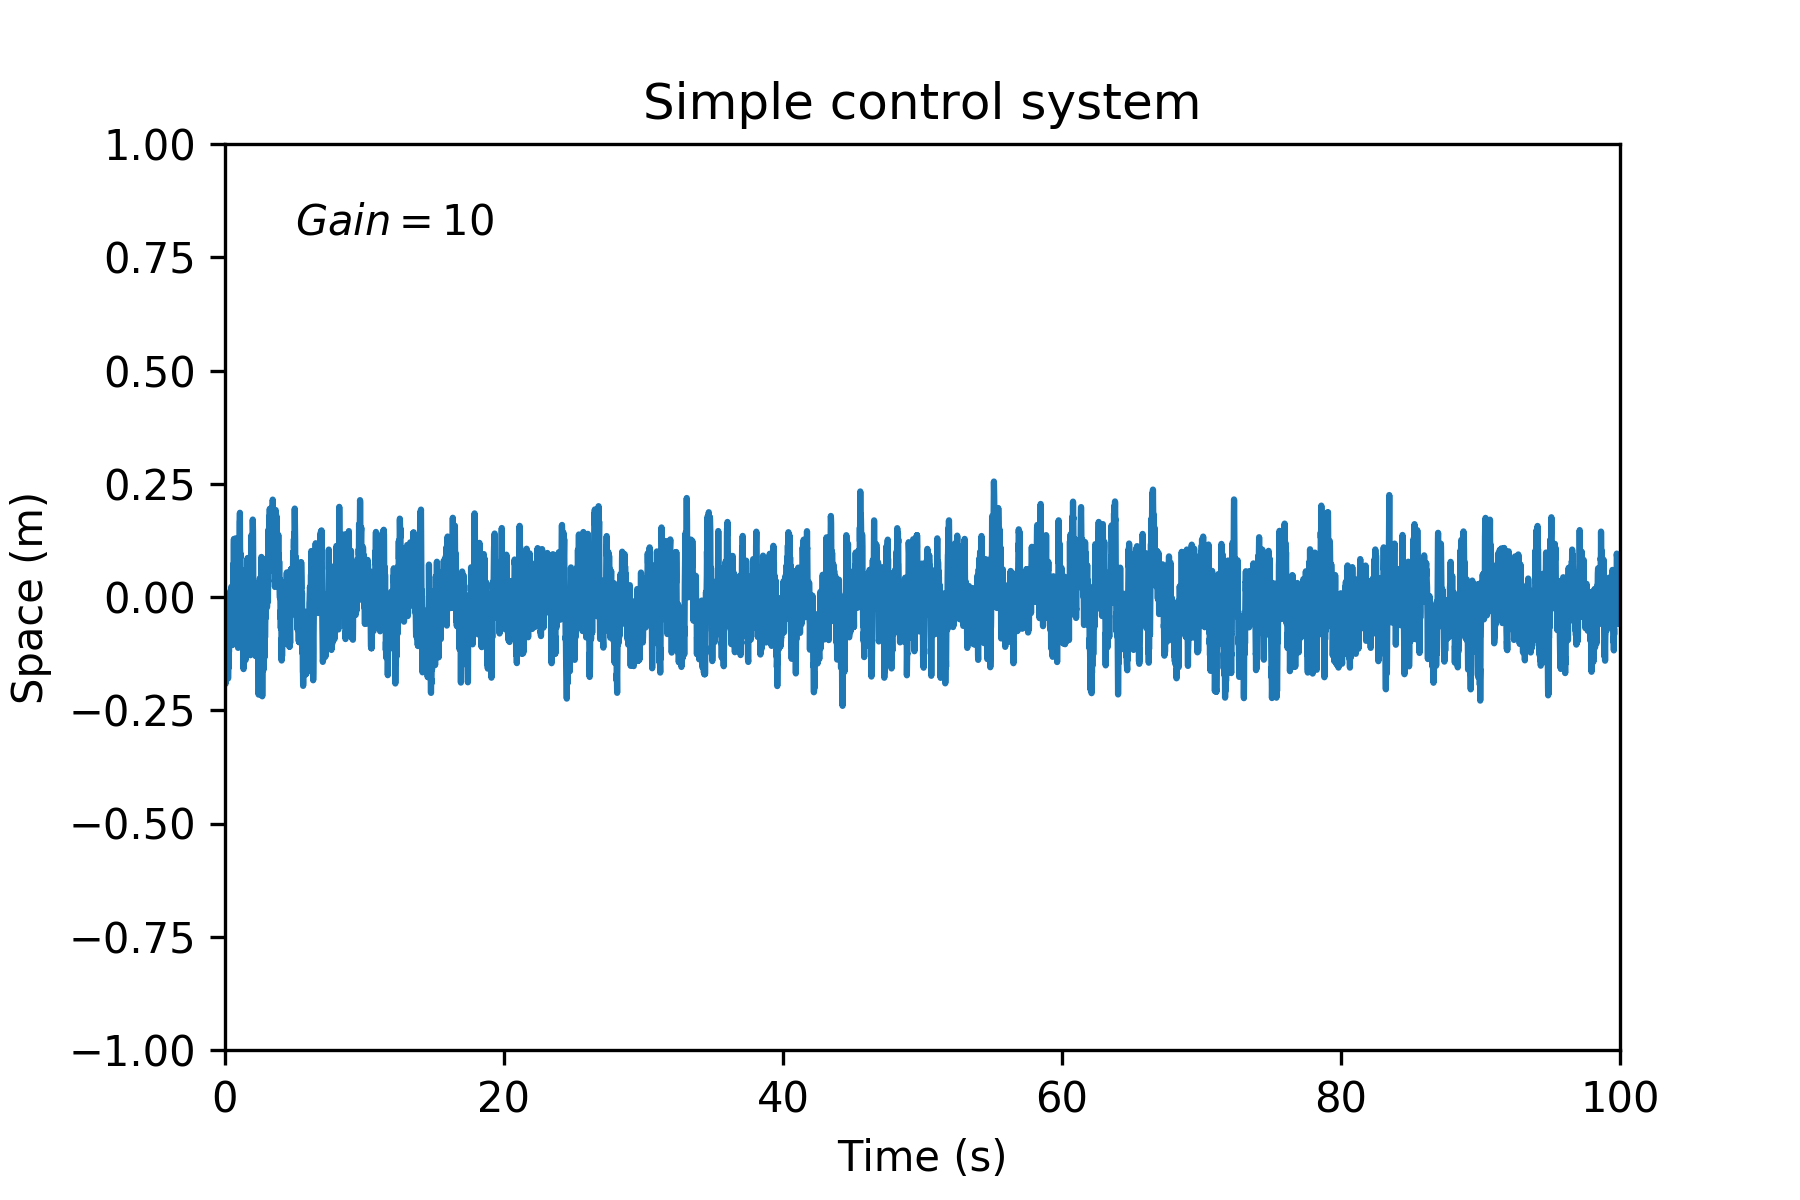
\includegraphics[width=10cm]{Kalman-control-Gain10}       
	\caption{The same system as in Figure~\ref{Kalman-control-Gain1.fig} with $K=10$. The empirical costs are $J_1=5.8\ 10^{-3}$ and  $J_2=1.59$.}
	\label{Kalman-control-Gain10.fig}
\end{figure}

\paragraph{The Kalman filter}
Now, we introduce the equations of the Kalman filter, which we know are optimal to estimate $x_k$.
\begin{eqnarray}
\label{kalman-filter.eq1}
\hat{x}_0 &=& 0\\
\label{kalman-filter.eq2}
P_0 &=& \bar{P}_0\\
\label{kalman-filter.eq3}
\hat{x}^-_{k+1} &=& A \hat{x}_k + B u_k\\
\label{kalman-filter.eq4}
P^-_{k+1} &=& A P_k A + Q\\
\label{kalman-filter.eq5}
\hat{x}_{k+1} &=& \hat{x}^-_{k+1} + L_{k+1}\left(y_{k+1}-C\hat{x}^-_{k+1}\right)\\
\label{kalman-filter.eq6}
L_{k+1} &=& P^-_{k+1}C\left(CP^-_{k+1}C+R\right)^{-1}\\
\label{kalman-filter.eq7}
P_{k+1} &=& \left(1-L_{k+1}C\right)P^-_{k+1}
\end{eqnarray}
These equations can be found in any textbook on control and are almost true as is for multidimensional states and measures. The most striking here is that the filter works whatever the control.

There is not much difference with Equation~(\ref{kalman-Pcontrol.eq}) in our control model, except that we take the best estimate:
\begin{equation}
\label{kalman-Pcontrol.eq2}
	u_k = -K \hat{x}_k
\end{equation}

This leads to the result of Figure~\ref{Kalman-TrueControl-Gain100.fig}. The precision is better than our previous best control (that was obtained for a lower gain) and the control cost is much lower than the control with same gain but based on Equation~(\ref{kalman-Pcontrol.eq}). Empirically, one sees that this gain is the optimal value in term of precision. As we are curious, we also vary the gain and we get the following results: for $K=10$, $J_1=8\ 10^{-3}$ and  $J_2=0.53$; for $K=1$, $J_1=0.072$ and  $J_2=0.069$. So we see that for lower gains (and this is much closer to realistic values), the precision is not much improved and the control cost improvement is noticeable mainly for high gains. Again, this certainly means we are missing some concepts. And here what we are missing is the notion of a better feedback control: the proportional control is too simple to be optimal. We could try a PID (Proportional-Integral-Derivative) or other controls (e.g. with pole placement), but in any case we learned that a Kalman filter allow to reduce the noise in the estimation of the state $x_k$.


\begin{figure}[htb]
	\centering
	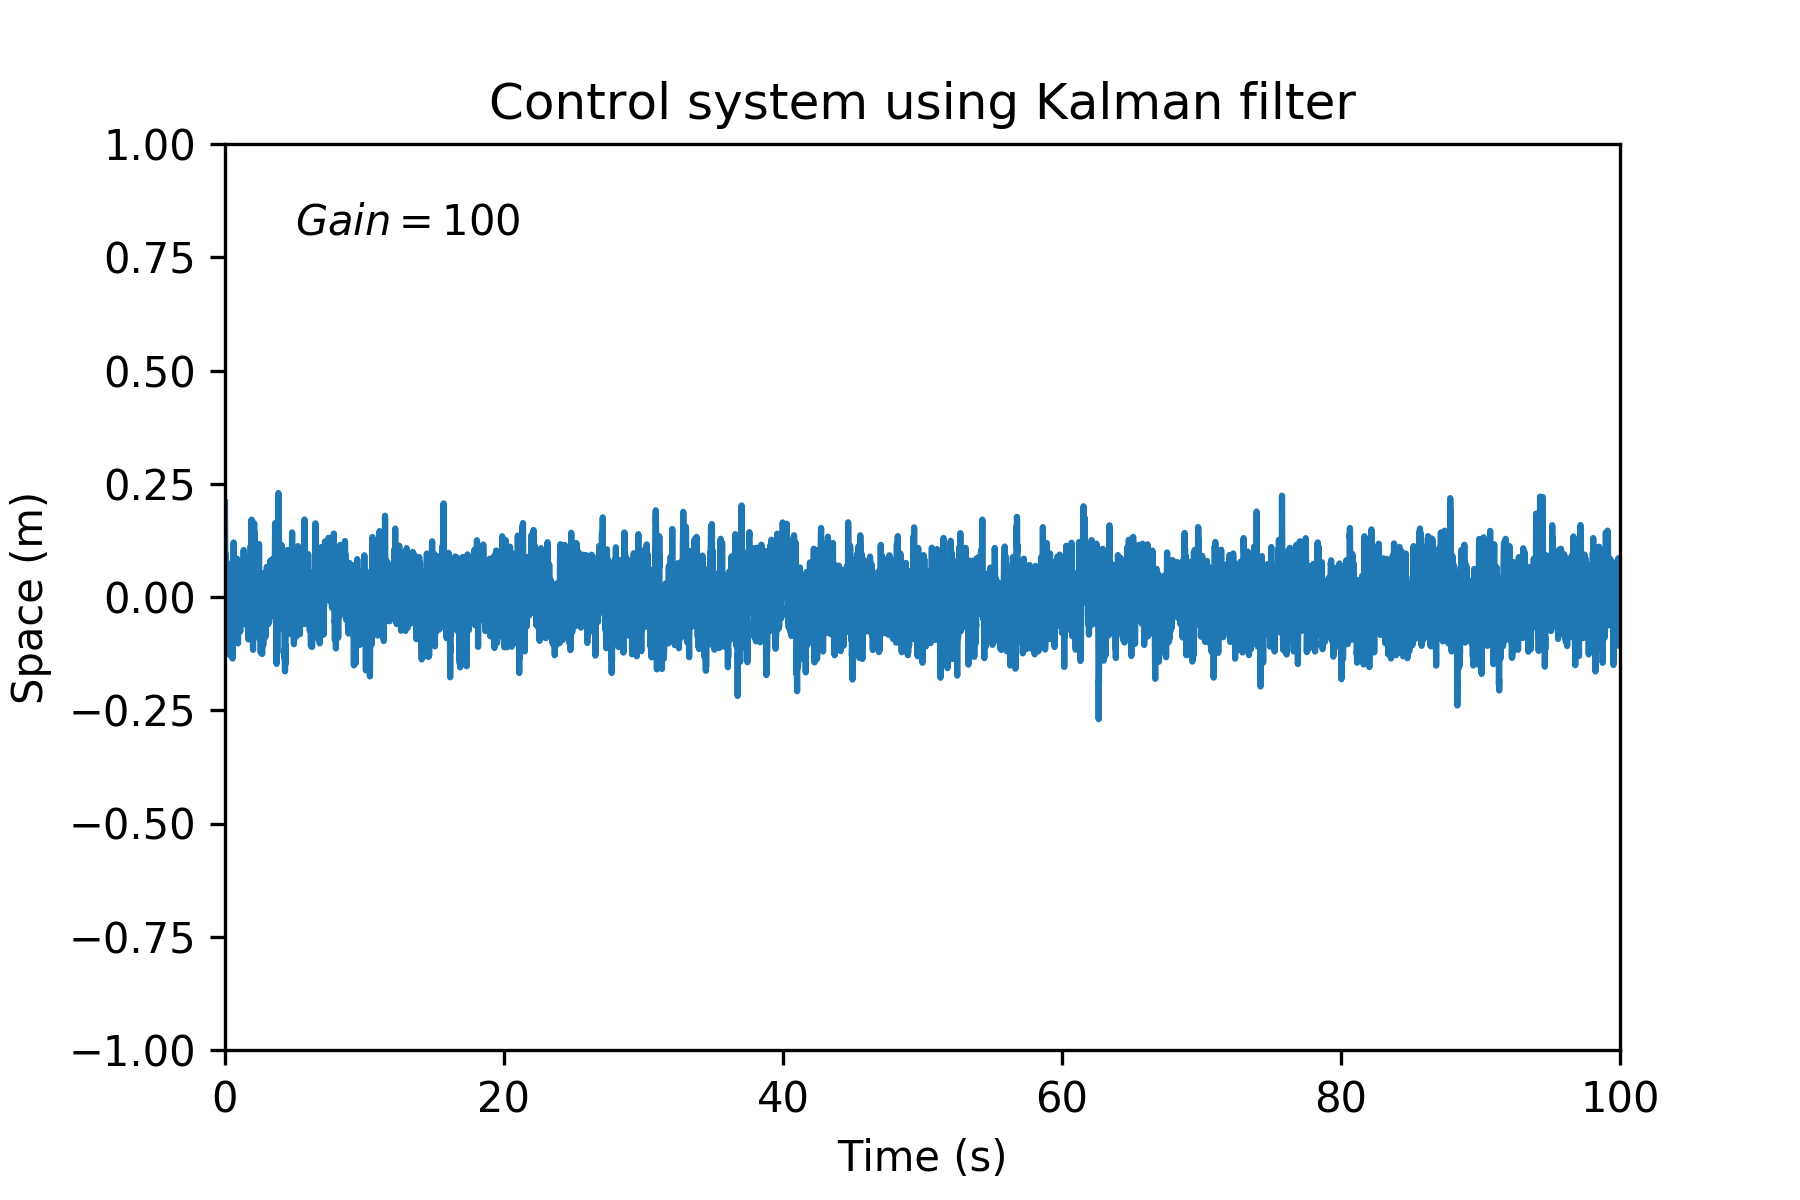
\includegraphics[width=10cm]{Kalman-TrueControl-Gain100}       
	\caption{The system with a proportional control based on Kalman filter with $K=100.1$. The empirical costs are $J_1=3.77\ 10^{-3}$ and  $J_2=10.2$.}
	\label{Kalman-TrueControl-Gain100.fig}
\end{figure}

In conclusion, note that what we learned practically about estimates, noise reduction and control are very general concepts that can be adapted to many situations, including PDEs. However, it generally requires some know-how to apply these notions.